\documentclass[10pt]{article}
% Supplementary material of MPCE_PSO_VNS.tex. Tables, figures, sections, algorithms and equations are numbered
% S1, S2, ...; the main text refers to them through xr (\externaldocument), so the numbering always matches.
% The generated tables come from analysis/mpce_supplementary.tex (written by analysis/mpce_results.py).
% Build: sh analysis/build_mpce_paper.sh (compiles this file and the main text alternately).
\usepackage[a4paper,margin=2cm]{geometry}
\usepackage{amsmath,amssymb}
\usepackage{algorithm}
\usepackage{algpseudocode}
\usepackage{booktabs}
\usepackage{graphicx}
\usepackage{multirow}
\usepackage{array}
\usepackage{xcolor}
\usepackage{url}
\usepackage[section]{placeins}
\usepackage{xr}
\externaldocument[M-]{MPCE_PSO_VNS}

\newcommand{\TBD}[1]{\textcolor{red}{[TBD\ifx\relax#1\relax\else: #1\fi]}}
\newcommand{\pipefig}[3]{\IfFileExists{#2}{\includegraphics[width=#1]{#2}}%
{\fbox{\parbox[c][#3][c]{\dimexpr#1-2\fboxsep-2\fboxrule\relax}{\centering\TBD{figure {\ttfamily\detokenize{#2}} not yet generated}}}}}

\renewcommand{\thetable}{S\arabic{table}}
\renewcommand{\thefigure}{S\arabic{figure}}
\renewcommand{\thealgorithm}{S\arabic{algorithm}}
\renewcommand{\theequation}{S\arabic{equation}}
\renewcommand{\thesection}{S-\Roman{section}}
\renewcommand{\thesubsection}{\thesection.\Alph{subsection}}
\setcounter{totalnumber}{6}\setcounter{topnumber}{4}\renewcommand{\topfraction}{0.95}\renewcommand{\textfraction}{0.05}
\renewcommand{\floatpagefraction}{0.6}

\title{Supplementary Material for\\ ``A Two-Phase Particle Swarm and Variable Neighborhood Search Algorithm\\ for Continuous Wind Farm Layout Optimization''}
\author{Prince Solanki, Pulkit Dwivedi, Vanita Garg, and Vinay Shukla}
\date{}

\begin{document}
\maketitle

\noindent Tables, figures, sections, algorithms and equations of this document are numbered S1, S2, \ldots; references without the prefix S (e.g., Table~\ref{M-tab:friedman68} or \eqref{M-eq:penalty}) point to the main text. Unless stated otherwise, all runs use 30 seed-paired runs of 6,030 objective calls, and the method names are those of the main text (PSO: constriction coefficients~\eqref{M-eq:constriction}).

\section{Model Details}
\label{sec:S-model}

\begin{figure}[!htb]
\centering
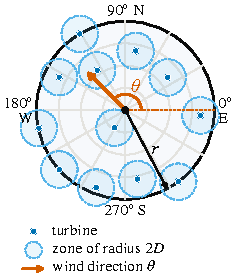
\includegraphics[width=0.5\textwidth]{figures_final/fig_wind_farm.pdf}
\caption{Circular wind farm of radius $r$. The wind direction $\theta$ (direction the wind blows towards) is measured counter-clockwise from east. The points show an optimized layout for 12 turbines in the 750-m farm (Wind Data Set~I); the shaded discs have radius $2D$, so two discs touch when their turbines are exactly $4D$ apart.}
\label{fig:S-farm}
\end{figure}
\begin{figure}[!htb]
\centering
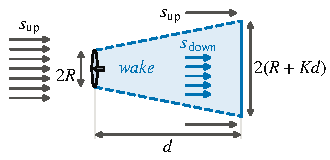
\includegraphics[width=0.55\textwidth]{figures_final/fig_wake_model.pdf}
\caption{Jensen wake behind a rotor of radius $R$ (schematic, not to scale). The wake widens linearly with the spreading constant $K$, so that its width at the downstream distance $d$ is $2(R+Kd)$, and the wind speed inside it drops from $s_{\text{up}}$ to $s_{\text{down}}$.}
\label{fig:S-wake}
\end{figure}
\begin{figure}[!htb]
\centering
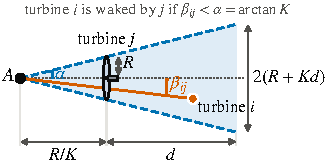
\includegraphics[width=0.55\textwidth]{figures_final/fig_half_cone.pdf}
\caption{Wake half cone of turbine $j$ (schematic, $K$ exaggerated). The virtual vertex $A$ lies a distance $R/K$ upstream of the rotor, the half-cone angle is $\alpha=\arctan K$, and a downstream turbine $i$ lies in the wake of $j$ when $\beta_{ij}<\alpha$.}
\label{fig:S-halfcone}
\end{figure}

\subsection{Discrete Form of the Expected Power}
\label{sec:S-power}
Following~\cite{Kusiak2010}, the integrals of \eqref{M-eq8} are evaluated with a Riemann sum. The wind direction is divided into bins $\theta_0 = 0^\circ, \theta_1, \ldots, \theta_{N_\theta} = 360^\circ$ with probabilities $p_l$, and the speed range between $s_{\text{cut-in}}$ and $s_{\text{rated}}$ into bins $s_0 = s_{\text{cut-in}}, s_1, \ldots, s_{N_s} = s_{\text{rated}}$. With $\bar\theta_l=(\theta_{l-1}+\theta_l)/2$ and $W_i(s,\theta)=\exp\{-[s/\psi_i(\theta)]^{\zeta(\theta)}\}$,
\begin{equation}
\begin{split}
E(P_i) ={}& \sum_{l=1}^{N_\theta} (\theta_l - \theta_{l-1})\, p_l \Bigg\{ P_{\text{rated}}\, W_i(s_{\text{rated}},\bar\theta_l)
+\lambda_1 \sum_{q=1}^{N_s} \frac{s_{q-1} + s_q}{2}\left[W_i(s_{q-1},\bar\theta_l)-W_i(s_q,\bar\theta_l)\right]\\
&+ \lambda_0 \left[W_i(s_{\text{cut-in}},\bar\theta_l)-W_i(s_{\text{rated}},\bar\theta_l)\right] \Bigg\}.
\end{split}
\label{eq:S-power}
\end{equation}
Like the earlier studies, we keep the bin-width factor $(\theta_l-\theta_{l-1})$. Because all 24 direction bins are $15^\circ$ wide and $\sum_l p_l=1$, the objective equals 15 times the expected farm power in kW, and $\mathrm{AEP}\,[\mathrm{MWh}] = (\text{objective}/15)\times 8.76$. The linear part of the power curve is $-7.0$~kW at 3.5~m/s and zero at 3.55~m/s.

\subsection{Gaussian Wake Model Used for the Re-Evaluation}
\label{sec:S-gauss}
For the re-evaluation of Section~\ref{M-sec:powercurve}, the deficit of the Jensen model is replaced by the Gaussian wake model of Bastankhah and Port\'e-Agel~\cite{Bastankhah2014},
\begin{equation}
\begin{split}
\Delta_{ij}&=\Bigl(1-\sqrt{1-C_T/(8\sigma^2/D^2)}\Bigr)\exp\!\bigl(-v_{ij}^2/(2\sigma^2)\bigr),\qquad
\sigma/D=K_{\rm G}\,d_{ij}/D+\epsilon,\\
\epsilon&=0.2\sqrt{\tfrac12(1+\sqrt{1-C_T})/\sqrt{1-C_T}},
\end{split}
\label{eq:S-gauss}
\end{equation}
for turbines $i$ downstream of $j$, with $K_{\rm G}=0.04$, the lateral offset $v_{ij}$ and downstream distance $d_{ij}$ of Section~\ref{M-sec:model}, and the same root-sum-square superposition and Weibull scaling as the benchmark.

\section{Salp Swarm Algorithm and Its Laplacian Variant}
\label{sec:S-ssa}
Algorithm~\ref{alg:S-ssa} summarizes SSA~\cite{Mirjalili2017} and LX-SSA~\cite{Solanki2023} as used in Phase~1 of SSA-VNS and LX-SSA-VNS and as stand-alone methods (Section~\ref{M-sec:ssa}). A follower moves to the midpoint $\tfrac{1}{2}(X_m^i+X_m^{i-1})$ between itself and the preceding salp; in LX-SSA it also forms the Laplace candidate~\eqref{M-eq:laplace} and keeps the better of the two, so that one LX-SSA iteration costs $2N_p$ objective calls.

\begin{algorithm}[!htb]
\caption{SSA and LX-SSA (lines marked LX: LX-SSA only)}
\label{alg:S-ssa}
\begin{algorithmic}[1]
\State Draw and evaluate $N_p$ salps; sort them and set the best as food source $\mathbf H$.
\For{$t=1$ to $T$}
    \State Update $\xi_1=2\exp[-(4t/T)^2]$.
    \For{salp $i=1,\ldots,N_p$}
        \If{$i\le N_p/2$}
            \State Update leader $i$ using \eqref{M-eq:leader}.
        \Else
            \State Form the follower candidate $\tfrac{1}{2}(\mathbf X^i+\mathbf X^{i-1})$.
            \State LX: form $\mathbf Y^i$ using \eqref{M-eq:laplace}, evaluate both candidates and keep the better one.
        \EndIf
    \EndFor
    \State Apply box repair, evaluate $F_p$ for the population, sort it, and update $\mathbf H$.
\EndFor
\State \Return $\mathbf H$.
\end{algorithmic}
\end{algorithm}

\section{Per-Case Results and Additional Tables}
\label{sec:S-tables}
Tables~\ref{tab:res-1-500}--\ref{tab:res-2-1000} give the per-case results of the main comparison; the remaining tables give the minimum-spacing re-optimization, the full case-level statistics, the coordinates of the best layouts, the computational cost and the per-case values of the budget-split, initialization, budget, Horns Rev~1, IEA37 and robustness studies of the main text. All tables in this section are generated by \texttt{analysis/mpce\_results.py}.

%% generated by mpce_results.py -- do not edit by hand
%% Supplementary tables (per-case results); requires booktabs, graphicx
\begin{table*}[!t]
\centering
\caption{Data Set I, 500-m farm: benchmark objective, mean (SD) over the feasible runs of 30 seed-paired runs at 6,030 objective calls. Bold: highest mean among the methods with at least 15 feasible runs. A superscript gives the number of feasible runs when fewer than 30; ``--'' means no feasible run.}
\label{tab:res-1-500}
\scriptsize\setlength{\tabcolsep}{2pt}
\resizebox{\textwidth}{!}{%
\begin{tabular}{ccccccccc}
\toprule
$N$ & Ideal & SSA-VNS & SSA & LX-SSA & PSO & DE & VNS & MS-SLSQP \\
\midrule
2 & 28091.5 & \textbf{28091.5 (0.0)} & \textbf{28091.5 (0.0)} & \textbf{28091.5 (0.0)} & \textbf{28091.5 (0.0)} & \textbf{28091.5 (0.0)} & \textbf{28091.5 (0.0)} & 28087.2 (4.6) \\
3 & 42137.2 & 42128.5 (10.7) & 42114.9 (10.3) & 42114.8 (14.2) & 42124.7 (8.5) & 42130.7 (8.8) & \textbf{42131.6 (9.7)} & 42116.0 (10.1) \\
4 & 56182.9 & 56101.8 (25.3) & 56086.8 (19.8) & 56078.8 (22.6) & 56094.3 (13.3) & 56092.8 (29.8) & \textbf{56106.1 (21.7)} & 56063.2 (30.9) \\
5 & 70228.7 & 69967.2 (159.2) & 69994.0 (34.0) & 69972.6 (72.0) & \textbf{70010.5 (27.2)} & 69960.5 (78.6) & 69876.9 (199.8) & 69930.5 (113.0) \\
6 & 84274.4 & \textbf{83780.8 (213.2)} & 83535.6 (372.5) & 83544.9 (465.3) & 83775.8 (154.1) & 83326.7 (761.5) & 83299.3 (524.5) & 83601.4 (213.1) \\
7 & 98320.2 & 96529.9 (794.9) & 96757.0 (692.4) & 96380.6 (1013.8) & 96935.0 (485.2) & 95903.3 (1316.3)$^{15}$ & 96967.1 (590.6) & \textbf{97037.0 (484.3)} \\
8 & 112365.9 & 109316.4 (1117.4) & 109172.6 (1362.4) & 108258.3 (1704.3)$^{28}$ & 108616.6 (1480.8)$^{24}$ & 107632.7 (1592.8)$^{2}$ & 109493.5 (2035.2) & \textbf{110226.6 (585.5)} \\
9 & 126411.6 & 121985.3 (1201.8) & 120043.1 (2755.8)$^{25}$ & 119134.2 (2666.4)$^{21}$ & 117175.2 (7148.7)$^{2}$ & --$^{0}$ & 122259.2 (1232.0) & \textbf{123222.8 (812.6)}$^{28}$ \\
10 & 140457.4 & 134321.3 (1482.4)$^{26}$ & 132616.3 (2328.0)$^{12}$ & 130967.4 (3191.0)$^{13}$ & --$^{0}$ & 130994.8 (0.0)$^{1}$ & 133567.5 (1820.9) & \textbf{135461.0 (1291.9)} \\
\bottomrule
\end{tabular}}
\end{table*}

\begin{table*}[!t]
\centering
\caption{Data Set I, 750-m farm: benchmark objective, mean (SD) over the feasible runs of 30 seed-paired runs at 6,030 objective calls. Bold: highest mean among the methods with at least 15 feasible runs. A superscript gives the number of feasible runs when fewer than 30; ``--'' means no feasible run.}
\label{tab:res-1-750}
\scriptsize\setlength{\tabcolsep}{2pt}
\resizebox{\textwidth}{!}{%
\begin{tabular}{ccccccccc}
\toprule
$N$ & Ideal & SSA-VNS & SSA & LX-SSA & PSO & DE & VNS & MS-SLSQP \\
\midrule
2 & 28091.5 & \textbf{28091.5 (0.0)} & \textbf{28091.5 (0.0)} & \textbf{28091.5 (0.0)} & \textbf{28091.5 (0.0)} & \textbf{28091.5 (0.0)} & \textbf{28091.5 (0.0)} & 28091.0 (1.6) \\
3 & 42137.2 & 42137.0 (1.0) & 42134.4 (4.1) & 42134.2 (4.8) & 42137.0 (1.1) & 42136.8 (1.5) & \textbf{42137.2 (0.0)} & 42132.3 (5.0) \\
4 & 56182.9 & 56162.3 (13.6) & 56153.8 (17.9) & 56149.9 (14.0) & 56160.0 (14.2) & 56146.9 (17.5) & \textbf{56167.0 (13.8)} & 56137.1 (16.4) \\
5 & 70228.7 & \textbf{70150.9 (25.4)} & 70122.2 (26.3) & 70118.1 (28.6) & 70135.0 (22.6) & 70083.9 (31.7) & 70125.8 (47.0) & 70100.5 (42.3) \\
6 & 84274.4 & \textbf{84095.6 (36.9)} & 84035.2 (58.4) & 84033.5 (58.3) & 84059.1 (42.0) & 83948.2 (74.1) & 84029.2 (141.3) & 83947.6 (95.9) \\
7 & 98320.2 & \textbf{97910.8 (164.8)} & 97875.2 (169.3) & 97840.0 (167.7) & 97872.3 (131.8) & 97479.1 (285.1) & 97774.4 (232.6) & 97710.2 (204.8) \\
8 & 112365.9 & \textbf{111683.9 (282.2)} & 111506.5 (334.5) & 111374.0 (460.8) & 111448.4 (551.6) & 110595.8 (445.6) & 111411.4 (493.5) & 111296.2 (217.8) \\
9 & 126411.6 & \textbf{125207.2 (539.4)} & 124756.2 (610.5) & 124698.0 (960.4) & 124550.0 (794.2) & 121674.9 (2276.5)$^{23}$ & 124780.0 (716.8) & 124818.4 (466.3) \\
10 & 140457.4 & \textbf{138304.3 (685.9)} & 137817.6 (1160.1) & 137748.6 (1116.3) & 137036.8 (1051.3)$^{28}$ & 134937.7 (998.5)$^{4}$ & 138170.4 (764.7) & 138184.7 (595.3) \\
11 & 154503.1 & 151286.3 (1117.4) & 150404.1 (1042.2)$^{29}$ & 149863.8 (1886.6)$^{29}$ & 149356.6 (1849.0)$^{20}$ & 148555.7 (1134.8)$^{3}$ & 151004.2 (1339.0) & \textbf{151352.9 (560.2)} \\
12 & 168548.8 & 164279.2 (1284.1) & 162903.5 (1685.8) & 161630.5 (1988.2)$^{28}$ & 160854.7 (2108.4)$^{7}$ & --$^{0}$ & 163712.4 (1575.6) & \textbf{164663.8 (674.6)} \\
\bottomrule
\end{tabular}}
\end{table*}

\begin{table*}[!t]
\centering
\caption{Data Set I, 1000-m farm: benchmark objective, mean (SD) over the feasible runs of 30 seed-paired runs at 6,030 objective calls. Bold: highest mean among the methods with at least 15 feasible runs. A superscript gives the number of feasible runs when fewer than 30; ``--'' means no feasible run.}
\label{tab:res-1-1000}
\scriptsize\setlength{\tabcolsep}{2pt}
\resizebox{\textwidth}{!}{%
\begin{tabular}{ccccccccc}
\toprule
$N$ & Ideal & SSA-VNS & SSA & LX-SSA & PSO & DE & VNS & MS-SLSQP \\
\midrule
2 & 28091.5 & \textbf{28091.5 (0.0)} & \textbf{28091.5 (0.0)} & \textbf{28091.5 (0.0)} & \textbf{28091.5 (0.0)} & \textbf{28091.5 (0.0)} & \textbf{28091.5 (0.0)} & 28091.3 (0.7) \\
3 & 42137.2 & \textbf{42137.2 (0.0)} & 42136.7 (1.6) & 42136.7 (1.4) & \textbf{42137.2 (0.0)} & \textbf{42137.2 (0.0)} & \textbf{42137.2 (0.0)} & 42135.9 (2.6) \\
4 & 56182.9 & \textbf{56180.0 (3.8)} & 56169.4 (9.2) & 56172.9 (7.8) & 56173.0 (6.8) & 56166.9 (8.4) & 56177.3 (8.6) & 56162.5 (10.5) \\
5 & 70228.7 & \textbf{70202.1 (15.9)} & 70174.0 (19.7) & 70183.3 (21.0) & 70182.6 (13.0) & 70148.7 (22.4) & 70193.3 (24.5) & 70151.4 (32.7) \\
6 & 84274.4 & \textbf{84175.9 (36.0)} & 84149.9 (29.7) & 84142.7 (23.5) & 84152.3 (22.2) & 84096.1 (24.0) & 84170.0 (49.5) & 84087.4 (92.6) \\
7 & 98320.2 & \textbf{98128.4 (59.9)} & 98084.7 (47.0) & 98078.4 (82.1) & 98083.0 (35.8) & 97942.3 (67.9) & 98064.6 (118.7) & 97955.8 (136.6) \\
8 & 112365.9 & \textbf{112008.3 (131.2)} & 111947.1 (125.7) & 111924.6 (164.7) & 111915.5 (125.3) & 111608.3 (168.9) & 111862.5 (246.1) & 111688.0 (181.9) \\
9 & 126411.6 & \textbf{125842.0 (277.4)} & 125761.1 (168.4) & 125701.5 (265.4) & 125531.1 (324.5) & 124996.3 (282.9) & 125589.7 (312.6) & 125366.6 (282.7) \\
10 & 140457.4 & \textbf{139561.7 (359.4)} & 139348.0 (433.0) & 139354.2 (388.5) & 139018.6 (478.6) & 137969.0 (623.0) & 139290.3 (447.7) & 139031.6 (341.6) \\
11 & 154503.1 & \textbf{153184.6 (292.3)} & 152825.1 (385.8) & 152736.8 (558.8) & 152337.8 (768.8)$^{29}$ & 150189.7 (1068.9)$^{29}$ & 153010.5 (393.8) & 152445.9 (402.0) \\
12 & 168548.8 & \textbf{166530.1 (760.0)} & 166091.9 (816.6) & 165814.4 (827.9) & 165072.5 (1367.5)$^{28}$ & 162390.4 (1765.9)$^{17}$ & 166510.6 (669.8) & 166188.4 (681.0) \\
13 & 182594.6 & \textbf{179973.5 (642.1)} & 179101.5 (1028.9) & 178913.6 (967.4) & 177302.0 (2352.6)$^{22}$ & 174763.4 (1389.6)$^{4}$ & 179762.6 (1091.2) & 179465.2 (506.2) \\
14 & 196640.3 & \textbf{193260.8 (939.8)} & 192235.7 (1504.8) & 191046.6 (1754.6) & 190385.1 (1544.4)$^{18}$ & --$^{0}$ & 192874.6 (1745.6) & 192677.8 (595.4) \\
15 & 210686.1 & \textbf{207119.3 (639.3)} & 204777.6 (1420.5) & 203681.8 (1899.5)$^{29}$ & 201985.5 (1678.3)$^{9}$ & --$^{0}$ & 206486.7 (1093.6) & 206059.6 (761.8) \\
\bottomrule
\end{tabular}}
\end{table*}

\begin{table*}[!t]
\centering
\caption{Data Set II, 500-m farm: benchmark objective, mean (SD) over the feasible runs of 30 seed-paired runs at 6,030 objective calls. Bold: highest mean among the methods with at least 15 feasible runs. A superscript gives the number of feasible runs when fewer than 30; ``--'' means no feasible run.}
\label{tab:res-2-500}
\scriptsize\setlength{\tabcolsep}{2pt}
\resizebox{\textwidth}{!}{%
\begin{tabular}{ccccccccc}
\toprule
$N$ & Ideal & SSA-VNS & SSA & LX-SSA & PSO & DE & VNS & MS-SLSQP \\
\midrule
2 & 14630.8 & \textbf{14630.8 (0.0)} & \textbf{14630.8 (0.0)} & \textbf{14630.8 (0.0)} & \textbf{14630.8 (0.0)} & \textbf{14630.8 (0.0)} & \textbf{14630.8 (0.0)} & 14626.0 (5.6) \\
3 & 21946.1 & 21907.1 (18.9) & 21900.9 (11.1) & 21899.7 (9.5) & 21901.5 (6.3) & 21901.2 (5.5) & \textbf{21932.3 (17.2)} & 21888.8 (45.5) \\
4 & 29261.5 & 29067.5 (60.7) & 29028.7 (93.8) & 29004.2 (87.4) & \textbf{29077.9 (64.5)} & 29044.2 (61.5) & 29070.8 (94.1) & 28998.9 (104.2) \\
5 & 36576.9 & 35958.0 (130.6) & 35918.9 (74.0) & 35880.1 (168.6) & \textbf{35959.4 (119.0)} & 35789.6 (193.8) & 35878.2 (160.9) & 35896.9 (110.0) \\
6 & 43892.3 & \textbf{42638.7 (198.9)} & 42444.3 (224.5) & 42512.1 (227.9) & 42568.5 (159.7) & 42257.5 (374.9) & 42560.3 (202.5) & 42590.7 (236.0) \\
7 & 51207.6 & 49008.6 (239.7) & 48887.9 (304.1) & 48626.5 (340.5) & 48885.9 (278.3) & 48203.9 (767.8)$^{15}$ & \textbf{49032.1 (314.4)} & 49007.9 (208.2) \\
8 & 58523.0 & 55274.9 (503.7) & 54900.5 (471.3) & 54699.5 (620.7)$^{28}$ & 54693.1 (404.3)$^{24}$ & 54451.3 (618.7)$^{2}$ & 55182.8 (738.6) & \textbf{55457.2 (287.3)} \\
9 & 65838.4 & 61380.0 (541.4) & 60581.0 (844.8)$^{25}$ & 59963.3 (652.2)$^{21}$ & 61035.6 (137.9)$^{2}$ & --$^{0}$ & 61166.8 (574.8) & \textbf{61457.0 (370.7)} \\
10 & 73153.8 & 67106.6 (779.5)$^{25}$ & 65880.7 (761.6)$^{12}$ & 65868.7 (586.0)$^{13}$ & --$^{0}$ & 64240.2 (0.0)$^{1}$ & 67056.0 (749.1) & \textbf{67288.3 (300.1)}$^{29}$ \\
\bottomrule
\end{tabular}}
\end{table*}

\begin{table*}[!t]
\centering
\caption{Data Set II, 750-m farm: benchmark objective, mean (SD) over the feasible runs of 30 seed-paired runs at 6,030 objective calls. Bold: highest mean among the methods with at least 15 feasible runs. A superscript gives the number of feasible runs when fewer than 30; ``--'' means no feasible run.}
\label{tab:res-2-750}
\scriptsize\setlength{\tabcolsep}{2pt}
\resizebox{\textwidth}{!}{%
\begin{tabular}{ccccccccc}
\toprule
$N$ & Ideal & SSA-VNS & SSA & LX-SSA & PSO & DE & VNS & MS-SLSQP \\
\midrule
2 & 14630.8 & \textbf{14630.8 (0.0)} & \textbf{14630.8 (0.0)} & \textbf{14630.8 (0.0)} & \textbf{14630.8 (0.0)} & \textbf{14630.8 (0.0)} & \textbf{14630.8 (0.0)} & 14630.4 (1.5) \\
3 & 21946.1 & \textbf{21946.1 (0.0)} & 21940.0 (8.2) & 21937.3 (8.1) & 21943.2 (5.4) & 21942.5 (5.8) & \textbf{21946.1 (0.0)} & 21938.2 (12.2) \\
4 & 29261.5 & 29210.5 (34.5) & 29182.5 (36.2) & 29201.4 (25.7) & 29213.0 (20.4) & 29195.3 (26.2) & \textbf{29227.3 (29.9)} & 29179.0 (59.2) \\
5 & 36576.9 & \textbf{36417.1 (67.3)} & 36332.0 (91.4) & 36366.8 (74.3) & 36400.0 (62.2) & 36277.7 (105.9) & 36389.7 (97.1) & 36283.6 (98.0) \\
6 & 43892.3 & \textbf{43500.1 (119.6)} & 43419.5 (153.1) & 43377.4 (175.7) & 43441.8 (107.5) & 43142.2 (144.8) & 43367.4 (201.2) & 43283.1 (153.3) \\
7 & 51207.6 & \textbf{50370.1 (169.6)} & 50264.8 (202.5) & 50095.4 (193.6) & 50188.2 (199.5) & 49696.6 (156.3) & 50180.2 (303.8) & 50164.7 (205.9) \\
8 & 58523.0 & \textbf{57033.9 (298.6)} & 56806.2 (303.6) & 56659.2 (332.0) & 56786.4 (311.8) & 56033.1 (331.4) & 56855.9 (391.5) & 56752.4 (256.7) \\
9 & 65838.4 & \textbf{63632.1 (366.8)} & 63291.6 (402.5) & 63252.7 (342.8) & 63180.2 (411.7) & 61970.8 (763.0)$^{23}$ & 63217.0 (515.4) & 63381.6 (322.9) \\
10 & 73153.8 & \textbf{70000.5 (393.6)} & 69520.3 (512.6) & 69480.7 (385.7) & 69159.6 (436.1)$^{28}$ & 68103.2 (423.7)$^{4}$ & 69930.2 (355.0) & 69972.9 (458.1) \\
11 & 80469.2 & 76265.0 (512.1) & 75742.5 (677.1)$^{29}$ & 75181.6 (681.1)$^{29}$ & 75199.6 (585.7)$^{20}$ & 74596.6 (476.3)$^{3}$ & 76099.7 (566.3) & \textbf{76284.4 (433.9)} \\
12 & 87784.5 & 82500.8 (492.0) & 81822.1 (625.7) & 81341.8 (792.1)$^{28}$ & 80936.3 (798.4)$^{7}$ & --$^{0}$ & 82368.6 (603.1) & \textbf{82867.2 (399.2)} \\
\bottomrule
\end{tabular}}
\end{table*}

\begin{table*}[!t]
\centering
\caption{Data Set II, 1000-m farm: benchmark objective, mean (SD) over the feasible runs of 30 seed-paired runs at 6,030 objective calls. Bold: highest mean among the methods with at least 15 feasible runs. A superscript gives the number of feasible runs when fewer than 30; ``--'' means no feasible run.}
\label{tab:res-2-1000}
\scriptsize\setlength{\tabcolsep}{2pt}
\resizebox{\textwidth}{!}{%
\begin{tabular}{ccccccccc}
\toprule
$N$ & Ideal & SSA-VNS & SSA & LX-SSA & PSO & DE & VNS & MS-SLSQP \\
\midrule
2 & 14630.8 & \textbf{14630.8 (0.0)} & \textbf{14630.8 (0.0)} & \textbf{14630.8 (0.0)} & \textbf{14630.8 (0.0)} & \textbf{14630.8 (0.0)} & \textbf{14630.8 (0.0)} & 14630.5 (1.0) \\
3 & 21946.1 & \textbf{21946.1 (0.0)} & 21945.6 (1.8) & 21945.3 (2.8) & 21945.8 (2.0) & \textbf{21946.1 (0.0)} & \textbf{21946.1 (0.0)} & 21943.5 (4.8) \\
4 & 29261.5 & 29247.6 (12.2) & 29232.5 (18.5) & 29228.0 (14.9) & 29243.3 (13.6) & 29225.9 (12.1) & \textbf{29253.1 (11.7)} & 29218.7 (24.2) \\
5 & 36576.9 & \textbf{36510.6 (35.3)} & 36485.9 (37.5) & 36468.2 (46.1) & 36486.0 (36.0) & 36402.8 (39.4) & 36498.4 (49.1) & 36432.0 (50.4) \\
6 & 43892.3 & \textbf{43736.8 (52.7)} & 43626.4 (74.5) & 43656.6 (73.3) & 43665.8 (65.6) & 43488.5 (69.7) & 43686.1 (101.2) & 43524.8 (86.8) \\
7 & 51207.6 & \textbf{50800.0 (120.6)} & 50731.8 (118.8) & 50727.3 (119.3) & 50739.2 (134.6) & 50442.7 (136.0) & 50696.0 (203.8) & 50582.5 (165.5) \\
8 & 58523.0 & \textbf{57883.4 (180.0)} & 57739.3 (142.0) & 57645.1 (186.6) & 57616.2 (157.7) & 57210.0 (191.8) & 57588.6 (311.3) & 57560.8 (206.6) \\
9 & 65838.4 & \textbf{64730.4 (233.0)} & 64476.4 (203.0) & 64428.7 (273.1) & 64308.4 (234.8) & 63790.1 (227.2) & 64430.8 (311.5) & 64419.1 (268.8) \\
10 & 73153.8 & \textbf{71541.9 (328.8)} & 71139.4 (336.8) & 71099.4 (266.9) & 70985.2 (314.4) & 70190.1 (286.9) & 71342.3 (339.4) & 71161.4 (275.8) \\
11 & 80469.2 & \textbf{78133.1 (465.6)} & 77697.5 (425.8) & 77561.6 (498.0) & 77501.2 (352.1)$^{29}$ & 75960.9 (577.6)$^{29}$ & 77948.1 (483.3) & 77812.4 (323.7) \\
12 & 87784.5 & \textbf{84647.1 (650.8)} & 84049.6 (660.3) & 83981.2 (515.0) & 83795.7 (565.1)$^{28}$ & 82211.6 (905.2)$^{17}$ & 84485.7 (606.8) & 84312.7 (466.3) \\
13 & 95099.9 & \textbf{91179.4 (556.4)} & 90267.0 (482.6) & 90303.5 (674.2) & 90139.1 (533.9)$^{22}$ & 88665.1 (496.0)$^{4}$ & 90787.8 (806.9) & 90837.9 (572.0) \\
14 & 102415.3 & \textbf{97590.4 (615.0)} & 96936.5 (669.3) & 96229.6 (1019.3) & 96266.2 (730.7)$^{18}$ & --$^{0}$ & 97079.1 (980.3) & 97276.4 (405.3) \\
15 & 109730.7 & \textbf{104035.3 (475.4)} & 102746.3 (827.8) & 102327.4 (838.7)$^{29}$ & 101804.8 (571.6)$^{9}$ & --$^{0}$ & 103777.6 (794.4) & 103853.3 (475.2) \\
\bottomrule
\end{tabular}}
\end{table*}


\section{Wind Data}
\label{sec:S-wind}
\begin{table}[!htb]
\centering
\caption{Wind Data Sets I and II: probability $p_l$ of direction bin $l$ ($[15(l-1),15l)^\circ$, direction the wind blows towards) and Weibull scale $\psi$; $\zeta=2$ in all bins.}
\label{tab:S-wind}
\scriptsize\setlength{\tabcolsep}{3.2pt}
\begin{tabular}{l*{12}{c}}
\toprule
Bin $l$ & 1 & 2 & 3 & 4 & 5 & 6 & 7 & 8 & 9 & 10 & 11 & 12 \\
\midrule
DS I: $p_l$ ($\psi=13$) & 0.000 & 0.010 & 0.010 & 0.010 & 0.010 & 0.200 & 0.600 & 0.010 & 0.010 & 0.010 & 0.010 & 0.010 \\
DS II: $\psi$ & 7.0 & 5.0 & 5.0 & 5.0 & 5.0 & 4.0 & 5.0 & 6.0 & 7.0 & 7.0 & 8.0 & 9.5 \\
DS II: $p_l$ & 0.0002 & 0.0080 & 0.0227 & 0.0242 & 0.0225 & 0.0339 & 0.0423 & 0.0290 & 0.0617 & 0.0813 & 0.0994 & 0.1394 \\
\midrule
Bin $l$ & 13 & 14 & 15 & 16 & 17 & 18 & 19 & 20 & 21 & 22 & 23 & 24 \\
\midrule
DS I: $p_l$ ($\psi=13$) & 0.010 & 0.010 & 0.010 & 0.010 & 0.010 & 0.010 & 0.010 & 0.010 & 0.010 & 0.010 & 0.010 & 0.000 \\
DS II: $\psi$ & 10.0 & 8.5 & 8.5 & 6.5 & 4.6 & 2.6 & 8.0 & 5.0 & 6.4 & 5.2 & 4.5 & 3.9 \\
DS II: $p_l$ & 0.1839 & 0.1115 & 0.0765 & 0.0080 & 0.0051 & 0.0019 & 0.0012 & 0.0010 & 0.0017 & 0.0031 & 0.0097 & 0.0317 \\
\bottomrule
\end{tabular}
\end{table}

\section{Comparison with Published Kusiak--Song Results}
\label{sec:S-literature}
The Kusiak--Song benchmark has been solved with an evolution strategy~\cite{Kusiak2010}, ant colony optimization~\cite{Eroglu2012}, particle filtering~\cite{Eroglu2013} and biogeography-based optimization~\cite{Bansal2017}. \TBD{author: literature table pending verification of the published values against the original papers (see analysis/literature\_values.md)}

\section{Additional Figures}
\label{sec:S-figs}
\begin{figure}[!htb]
\centering
\pipefig{\textwidth}{figures_mpce/convergence_max.pdf}{8cm}
\caption{Convergence of the eight methods of the main comparison for the largest $N$ of each farm: median (line) and interquartile range (band) of the best feasible wake loss over 30 runs versus objective calls.}
\label{fig:S-conv-max}
\end{figure}
\begin{figure}[!htb]
\centering
\pipefig{\textwidth}{figures_mpce/convergence_mid.pdf}{8cm}
\caption{As Fig.~\ref{fig:S-conv-max}, for the middle $N$ of each farm ($N=6$, 8 and 10 for $r=500$, 750 and 1000~m).}
\label{fig:S-conv-mid}
\end{figure}
\begin{figure}[!htb]
\centering
\pipefig{\textwidth}{figures_mpce/boxplots_max.pdf}{8cm}
\caption{Distribution of the wake loss of the feasible runs for the largest $N$ of each farm (number of feasible runs in parentheses when fewer than 30).}
\label{fig:S-box-max}
\end{figure}
\begin{figure}[!htb]
\centering
\pipefig{\textwidth}{figures_mpce/boxplots_mid.pdf}{8cm}
\caption{As Fig.~\ref{fig:S-box-max}, for the middle $N$ of each farm.}
\label{fig:S-box-mid}
\end{figure}
\begin{figure}[!htb]
\centering
\pipefig{\textwidth}{figures_mpce/feasibility_vs_n.pdf}{8cm}
\caption{Percentage of feasible runs versus the number of turbines.}
\label{fig:S-feas}
\end{figure}
\begin{figure}[!htb]
\centering
\pipefig{\textwidth}{figures_mpce/layouts_max.pdf}{9cm}
\caption{Best layout of all methods (squares) and best PSO-VNS layout (dots) for the largest $N$ of each farm; the coordinates are listed in Table~\ref{tab:coords}.}
\label{fig:S-layouts}
\end{figure}
\begin{figure}[!htb]
\centering
\pipefig{\textwidth}{figures_mpce/hr16.pdf}{7cm}
\caption{Horns Rev~1 16-turbine block: median best feasible AEP versus objective calls (left) and layouts (right).}
\label{fig:S-hr16}
\end{figure}
\begin{figure}[!htb]
\centering
\pipefig{\textwidth}{figures_mpce/iea37_convergence.pdf}{6cm}
\caption{IEA37 Case Study~1: median best feasible wake loss versus objective calls at the largest budget.}
\label{fig:S-iea37-conv}
\end{figure}

\begin{thebibliography}{9}
\bibitem{Kusiak2010} A. Kusiak and Z. Song, ``Design of wind farm layout for maximum wind energy capture,'' \textit{Renew. Energy}, vol. 35, no. 3, pp. 685--694, 2010.
\bibitem{Eroglu2012} Y. Ero\u{g}lu and S. U. Se\c{c}kiner, ``Design of wind farm layout using ant colony algorithm,'' \textit{Renew. Energy}, vol. 44, pp. 53--62, 2012.
\bibitem{Eroglu2013} Y. Ero\u{g}lu and S. U. Se\c{c}kiner, ``Wind farm layout optimization using particle filtering approach,'' \textit{Renew. Energy}, vol. 58, pp. 95--107, 2013.
\bibitem{Bansal2017} J. C. Bansal and P. Farswan, ``Wind farm layout using biogeography based optimization,'' \textit{Renew. Energy}, vol. 107, pp. 386--402, 2017.
\bibitem{Mirjalili2017} S. Mirjalili \textit{et al.}, ``Salp swarm algorithm: A bio-inspired optimizer for engineering design problems,'' \textit{Adv. Eng. Softw.}, vol. 114, pp. 163--191, 2017.
\bibitem{Solanki2023} P. Solanki and K. Deep, ``Laplacian salp swarm algorithm for continuous optimization,'' \textit{Int. J. Syst. Assur. Eng. Manag.}, 2023.
\bibitem{Bastankhah2014} M. Bastankhah and F. Port\'e-Agel, ``A new analytical model for wind-turbine wakes,'' \textit{Renew. Energy}, vol. 70, pp. 116--123, 2014.
\bibitem{Benavoli2016} A. Benavoli, G. Corani, and F. Mangili, ``Should we really use post-hoc tests based on mean-ranks?'' \textit{J. Mach. Learn. Res.}, vol. 17, no. 5, pp. 1--10, 2016.
\bibitem{Baker2019} N. F. Baker \textit{et al.}, ``Best practices for wake model and optimization algorithm selection in wind farm layout optimization,'' in \textit{Proc. AIAA SciTech Forum}, 2019, Paper AIAA 2019-0540.
\bibitem{IEA37repo} N. F. Baker \textit{et al.}, ``IEA Wind Task 37 wind farm layout optimization case studies: Case files and submitted results.'' [Online]. Available: \url{https://github.com/IEAWindTask37/iea37-wflo-casestudies}
\end{thebibliography}

\end{document}
